\subsection{Greedy Heuristic Path}\label{sec:greedy}
As mentioned in previous section finding an optimal solution to a path is an NP-complete problem. In this section a greedy heuristic approach is taken which solves the problem one edge at a time, instead of trying to give a solution to an entire path. The problem then becomes, which speed must we use for the current edge, in the interval of $v_{min}$ and $v_{max}$.

Given a path there are two probable cases when choosing the optimal speed to pass an edge:
\begin{enumerate}
	\item Driving is fastest
	\item Charging and driving is fastest
\end{enumerate}

The intuition is then to find which speed we want to drive and whether or not we should charge before driving. However, it might not be possible to drive at all, given the limited battery of the EV. The optimal speed when passing the edge $e_i$ = $(u_i, u_{i+1})$ without charging, can be found by solving this equation for $v$:
\[B_{cur} - D(e_i) * R_{CO}(v) = 0\] 
We call this speed $v_{opt}$. If $v_{opt}$ is lower than $v_{min}(e_i)$, there is not enough energy in the battery to drive from $u_i$ to $u_{i+1}$ and thus the time is set to $\infty$, indicating that just driving is not an option. If it is possible to drive the edge using only energy from the battery, the time it will take to pass the edge can be calculated as:
 \[T = \frac{D(e_i)}{v_{opt}} \] 
The time spent passing edge $e_i$ when charging and driving, is given by the following equation:
\begin{equation*}
\begin{aligned}
 & T(v,e_i) = \frac{D(e_i)}{v} + \frac{R_{CO}(v) * D(e_i) - B_{cur}}{charge_{rate}(u_{i})}
\end{aligned}
\end{equation*}
Where $v$ is the speed of the vehicle, $D(u_i, u_{i+1})$ is the distance between vertices $u_i$ and $u_{i+1}$, $R_{CO}(v)$ is the consumption rate of the EV, $B_{cur}$ is the current battery of the vehicle. Since we only charge exactly enough to pass an edge, there might be charging stations previous to $u_i$ which we could have charged more at, without exceeding the battery capacity. Therefore we want go back in history and charge at the best previous charging stations, until we have enough energy to pass edge $e_i$. This is done by $charge_{rate}(u_i)$ which gives the charge rate of the best charging station previous to $u_{i}$ or the charge rate of $u_i$ if $u_i$ is a better charging station than any of the charging stations prior to $u_i$. The charging stations that can be used, is of course only those which are within the EV's battery range.

The above equation yields a function of the form: $av^2 + bv + c$, due to the fact that $R_{CO}(v)$ is a quadratic function. $a$, $b$ and $c$ are some constants which are given by the instance of the vehicle. Represented in a Cartesian coordinate system, $T(v,(u_i, u_{i+1})))$ is a parabola, as can be seen in Figure \ref{fig:graph}, note that the graph is only defined for positive speeds larger than $0$ and can only be calculated if $charge_{rate}(u_{i+1})$ is larger than $0$. On the x-axis is the speed of the vehicle and on the y-axis is the time spent. The turning point of the graph represents the optimal speed to drive for the given edge, denoted as $v_{opt}(e)$. The turning point is easily calculated by finding a tangent line with a slope of $0$. If $v_{opt}(e)$ is smaller than $v_{min}(e)$, then $v_{min}(e)$ defines the optimal speed for the edge. Similarly if $v_{opt}(e)$ is larger than $v_{max}(e)$, $v_{max}(e)$ defines the optimal speed for the edge. If $v_{opt}(e) = v_{min}(e)$ there might be a possibility that driving and charging is not an option. 

\begin{figure}[!htb]
\label{fig:graph}
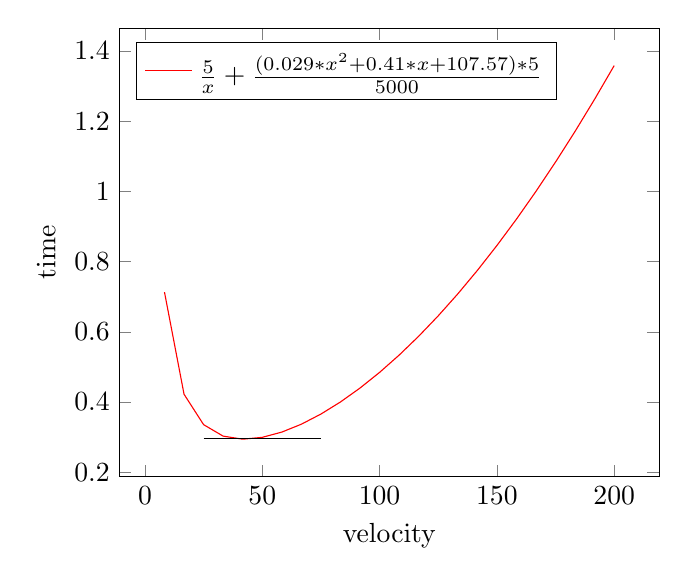
\begin{tikzpicture}
\begin{axis}[xlabel=velocity, ylabel=time,legend style={legend pos=north west}]
\addplot[draw=red,domain=0:200]{(5/x)+(((0.0286*x^2 + 0.4096*x + 107.57)*5)/5000)};
\addlegendentry{$\frac{5}{x}+\frac{(0.029*x^2 + 0.41*x + 107.57)*5}{5000}$}

\addplot[draw=black,domain=25:75]{0.295};
% \addplot[mark=*, domain=25:75] coordinates {(37,295)};
\end{axis}
\end{tikzpicture}% 
\caption{In this instance of $T(v,e_i)$, going from $u_i$ to $u_{i+1}$, we have a distance of $5 \si{\km}$ and a charge speed of $5 \si{\kW}$ on $u_i$. The optimal speed in this case is $42.12\si{\km\per\hour}$, and the total time is roughly 17 minutes to pass through the edge when driving and charging}
\label{fig:graph}
\end{figure}
Having the two ways of deciding the time it takes to pass an edge, we can formulate an algorithm which decides how to drive each local road segment:

\begin{algorithm}[!htb]
 \begin{algorithmic}[1]
  \Function{travel\_time}{$RN, u_1, u_2, EV$}
  	\State $e = (u_1, u_2)$
  	\State $v_{opt1} = solve1(v, e, EV.B_{cur}-RN.D(e)*EV.R_{CO}(v))$
  	\If{$ u_1.B_{cur} - RN.D(e)*EV.R_{CO}(v_{opt1}) < 0 $}
  		\State $time_1 = \infty$
  	\Else
 		\State $time_1 = RN.D(e) / v_{opt1}$
 		\State $energy\_used_{1} = RN.D(e)*EV.R_{CO}(v_{opt1})$
  	\EndIf
		\State $CS = charge_{rate}(u_1)$ 
  		\State $energy\_needed_{2} = \infty$
  		\State $energy = u_1.B_{cur}$
  		\State $time\_added = 0$
  		\State $time_2 = \infty$
  	\While{$energy\_needed_{2} > energy  \And  len(CS) \neq 0$}
  		\State $best_{CS} = extractmax(CS)$
  		\State $B_{possible} = best_{CS}.B_{possible}$
  		\State $charge\_rate = RN.R_{CH}(best_{CS})$
  		\State $v_{opt2} = solve2 (v, e,  RN.D(e)/v + (RN.D(e) * EV.R_{CO}(v)-energy)/charge\_rate))$ 
  		\State $energy\_needed_{2} = RN.D(e)*EV.R_{CO}(v_{opt2})$
  		\State $energy = energy + B_{possible}$
  		\If{$energy - energy\_needed_{2}) < 0$}
  			\State $time\_added = time\_added + (B_{possible} / charge\_rate)$
  			\State $CS.remove(0)$
  			\State $updateCS(CS)$
  		\EndIf	
  	\EndWhile
  	\If{$(energy - energy\_needed_{2}) < 0$}
  		\State $time_2 = (RN.D(e)/v_{opt2}) + (energy\_needed_{2}/charge\_rate) + time\_added$
  	\EndIf
  	\If{$time_1 = \infty \And time_2 = \infty$}
  		\State \Return $\infty, NIL, \infty$
  	\EndIf
  	\If{$time_1 \leq time_2$}
  		\State \Return $time_1, CS, energy\_used_1$
  	\Else
  		\State \Return $time_2, CS, energy\_used_2$
  	\EndIf
  \EndFunction
  \end{algorithmic}\label{alg:fastest_path}
\end{algorithm}

\todo[inline]{This algorithm... really?}

The $travel\_time$ function takes as input a road network $RN$, the two vertices which makes up the edge to be driven and the EV which is driving. The procedure utilizes a few helping functions, which we have not included for simplicity, we will however briefly explain them. The two solve functions $solve1$ and $solve2$ are function solvers specified for each of the cases and returns the optimal speed of the EV within the speed limit of the edges driven. The function $getCS(u_1)$ returns a list of charging stations. If $u_1$ is a charging stations with a higher charge rate than any charging station previous to $u_1$ then $u_1$ is returned. Otherwise $u_1$ is append to the list of charging stations previous to $u_1$, this ensure that the charging station with the best charge rate is always the first in the list of previous charging stations. 

The last function $updateCS(CS)$ finds a new best charging station and deletes all charging stations prior to it, this is need because the best charging station have been removed by $CS.remove(0)$. Lines 3-8 handles case 1: Driving using the battery already in the battery. Lines 9-26 handles case 2: Charging and driving. The while loop ranging from line 14 till 24 makes sure the EV always charge as much as possible, at the best previous charging station, but without allowing overcharging. The if statement on line 4 and 25 checks if a valid solution to the case is found, if so, the time for the case is calculated. Lines 27-32 checks if a solution is found and if so, which solution is better. Having a way to solve a single edge, the time of the path can be decided by looping through all edges form $e_1$ to $e_n$

The $travel\_time$ procedure can then be used to solve a path. One simply has to call it for each consecutive edge.


